
\documentclass[a4paper,norsk]{article}
\usepackage{preamble}
\usepackage{tabu}
\usepackage{color, colortbl}
\definecolor{LightCyan}{rgb}{0.88,1,1}


\begin{document}
\maketitle

\section{Exercise 1}
In these set of exercises we will study the Stokes problem defined as
\begin{align*}
-\Delta u + \nabla p = f \hspace{2mm} \text{in} \hspace{2mm} \Omega \\
\nabla \cdot v = 0 \hspace{2mm} \text{in} \hspace{2mm} \partial\Omega \\
u = g \hspace{2mm} \text{in} \hspace{2mm} \partial\Omega_N \\
\frac{\partial u}{\partial x} - pn = h \hspace{2mm} \text{in} \hspace{2mm} \partial\Omega_N\\
\end{align*}

First off we will define the weak formulation for the stokes problem. Let u $\in H_{D,g}^1$ and $p \in L^2$. Then
the stokes problem can be defined as
\begin{align*}
a(u, v) + b(p, v) = f(v) \hspace{2mm} v \in H_{D,0}^1 \\
b(q, u) = 0 \hspace{2mm} q \in L^2
\end{align*}
Where a and b defines the bilinear form, and f defines the linear form as

\begin{align*}
a(u, v) = \int \nabla u : \nabla v \hspace{1mm} dx \\
b(p, v) = \int p \nabla \cdot v \hspace{1mm} dx \\
f(v) = \int f v \hspace{1mm} dx + \int_{\Omega_N} h v \hspace{1mm} ds
\end{align*}

Further we will define to properties which will be usefull for solving the exercises \newline \newline
\textbf{Cauchy-Schwarts inequality} \\
Let V be a inner product space, then
\begin{align*}
 |\langle u \,, v \rangle| \hspace{1mm} \leq \hspace{1mm} ||u|| \cdot ||w|| \hspace{2mm} \forall \hspace{1mm} v,q \in V
\end{align*}
\newline
\textbf{Poincare's Inequality}
Let $v \in H_0^1(\Omega)$
\begin{align*}
||v||_{L^2(\Omega)} \leq C |v|_{H^1} (\Omega)
\end{align*}

\newpage
\subsection*{Exercise 7.1}
In this section we are to prove the conditions (7.14-7.16) from the course lecturenotes.
Starting off with the first
\textbf{Condition 7.14}
\begin{align*}
a(u_h, v_h) \leq C_1 ||u_n||_{V_n} ||v_n||_{V_n} \hspace{2mm} \forall u_n, v_n \in V_n
\end{align*}
As for in all of these conditions we will assume that $V_h \in H_0^1$, and for later conditions that$Q_h \in L^2$.
\newline
First off we write out the term $a(u_h, v_h)$, and we observe we can use the Cauchy-Schwarts inequality since
V is an inner product space.
\begin{align*}
a(u_h, v_h) = \int_\Omega \nabla u_h : \nabla v_h \hspace{1mm} dx  = \langle \nabla u_h \,, \nabla v_h \rangle \\
\langle \nabla u_h \,, \nabla v_h \rangle \leq |\langle \nabla u_h \,, \nabla v_h \rangle|_0
\leq ||\nabla u_h||_0 \cdot ||\nabla v_h||_0
\end{align*}
Now since we have defined that $u_h, v_h \in V_h \in H_0^1$ we can use the Poincare inequality. Since we know that the norms
are positive, we are allowed to square the norm. We get the following relations.

\begin{align*}
||\nabla u_h ||^2_{0} \leq ||u_h||^2_{1} = ||u_h||^2_{0} + ||\nabla u_h||^2_{0} \leq D |u_h|^2_{1} +  ||\nabla u_h||^2_{0} =
D ||\nabla u_h||^2_{0} +  ||\nabla u_h||^2_{0} \\
(D + 1) ||\nabla u_h||^2_{0} \leq C_1 ||u_h||^2_{1}
\end{align*}
The following can be showed for $||\nabla v_h ||^2_{0}$ aswell, hence it is clear that
\begin{align*}
||\nabla u_h ||_0 \cdot ||\nabla v_h ||_0 \leq C_1 ||u_h||_1 \cdot ||v_h||_1
\end{align*}

\textbf{Condition 7.15}
\begin{align*}
b(u_h, q_h) \leq C_2 ||u_h||_{V_h} ||q_h||_{Q_h} \hspace{2mm}  V_h \in H_0^1, \hspace{2mm} Q_h \in L^2,
\end{align*}
By direct insertion we get

\begin{align*}
b(u_h, q_h) = \int p \nabla \cdot v \hspace{1mm} dx = \langle p \,, \nabla \cdot u \rangle \leq | \langle p \,, \nabla \cdot u \rangle |_0
\end{align*}
Using the Cauchy-Schwarts inequality we can show that
\begin{align*}
| \langle q \,, \nabla \cdot u \rangle |_0 \leq ||q||_0 \cdot ||\nabla \cdot u||_0
\end{align*}
Hence, it holds to show that
\begin{align*}
  ||q||_0 \cdot ||\nabla \cdot u||_0 \leq C_2 ||u_h||_{1} ||q_h||_{0} \\
  ||\nabla \cdot u||_0 \leq C_2 ||u_h||_{1}
\end{align*}
We choose square the left side of the inequality and expand the norm, in hope of finding a term to
determine the upper bound of b. Applying the poincare inequality on line 2, we can determine that the bound must be
determined by some constant $C_2$
\begin{align*}
||\nabla \cdot u||_0^2 \leq ||u||_1^2 = ||u||_0^2 + ||\nabla u ||_0^2 \\
||u||_0^2 + ||\nabla u ||_0^2 \leq D |u|_1 + ||\nabla u||_0^2 = (D + 1)||\nabla u ||_0^2 = C_2||\nabla u ||_0^2
\end{align*}
Hence, to show the implied boundedness of b, it holds to show $||\nabla \cdot u||_0^2 \leq C_2||\nabla u ||_0^2$
For simplicity we write out the terms for the $R^2$ case, but the same proof can be showed for the general case $R^n$.

\begin{align*}
 ||\nabla \cdot u||_0^2 = \int \big(\frac{\partial^2 u}{\partial x^2} + \frac{\partial^2 v}{\partial y^2}\big)^2 \hspace{1mm} dx \\
 ||\nabla u||_0^2 = \int \big(\frac{\partial^2 u}{\partial x^2}\big)^2 + \big(\frac{\partial^2 u}{\partial y^2} \big)^2 +
 \big(\frac{\partial^2 v}{\partial x^2} \big)^2 + \big( \frac{\partial^2 v}{\partial y^2} \big)^2 \hspace{1mm} dx
\end{align*}
Remembering that since we are in a normed vector space V, the triangle inequality holds.
\begin{align*}
||x + y || \leq ||x|| + ||y|| \hspace{2mm} \forall x,y \in V
\end{align*}
Rearrangeing the terms we observe that
\begin{align*}
 ||\nabla \cdot u||_0^2 = \int \big(\frac{\partial^2 u}{\partial x^2} + \frac{\partial^2 v}{\partial y^2}\big)^2 \hspace{1mm} dx \\
 ||\nabla u||_0^2 = \int \big(\frac{\partial^2 u}{\partial x^2}\big)^2
 +  \big( \frac{\partial^2 v}{\partial y^2} \big)^2 \hspace{1mm} dx
 + \int \big(\frac{\partial^2 v}{\partial x^2} \big)^2 +
  \big(\frac{\partial^2 u}{\partial y^2} \big)^2  \hspace{1mm} dx \\
  \sqrt{ \int \big(\frac{\partial^2 u}{\partial x^2} + \frac{\partial^2 v}{\partial y^2}\big)^2 \hspace{1mm} dx }\leq
 \sqrt{ \int \big(\frac{\partial^2 u}{\partial x^2}\big)^2}
 + \sqrt{ \big( \frac{\partial^2 v}{\partial y^2} \big)^2 \hspace{1mm} dx }
\end{align*}
Hence $||\nabla \cdot u||_0^2 \leq C_2 ||\nabla u ||_0^2$, and the inequality holds.

\textbf{Condition 7.16, Coersivity of a}
\begin{align*}
 a(u_h, u_h) \geq C_3 ||u_h||_{V_h}^2 \hspace{2mm} \forall u_h \in V_h
\end{align*}
Expanding the $H^1$ norm of $u_h$, and applying the Cauchy-Schwarts inequality we find the relations

\begin{align*}
||u_h||_1^2 = ||u_h||_0^2 + ||\nabla u_h||_0^2 \leq C|u_h|_1^2 + ||\nabla u_h||_0^2 \\
= C||\nabla u_h||_0^2 + ||\nabla u_h||_0^2 = \big(C + 1\big)||\nabla u_h||_0^2 = C_3 ||\nabla u_h||_0^2 \\
\end{align*}
Dividing the constant on both sides of the inequality and let $C_3 = 1/C_3$ we get our final result which proofs the coersivity of a
\begin{align*}
C_3||u_h||_1^2 \leq ||\nabla u_h||_0^2 = \int \nabla u_h : \nabla u_h \hspace{1mm} dx = a(u_h, u_h)
\end{align*}

\newpage
\subsection{Exercise 7.6}
Looking on the poiseuille flow, we are to investigate if the anticipated convergence rates applies for the problem

\begin{align*}
-\Delta u - \nabla p = f \hspace{2mm} \text{in} \hspace{2mm} \Omega \\
\nabla \cdot u = 0 \hspace{2mm} \text{in} \hspace{2mm} \partial\Omega \\
\end{align*}
We will make use of the "manufactured solution" approach defining an analytical solution in $\Omega$ and finding the appropriate
source function f. By using hand calculations and verification of sympy we get.

\begin{align*}
 u = (sin(\pi y), cos(\pi x)); \hspace{4mm} p = sin(2 \pi x) \\
 f = (\pi^2 sin(\pi y) - 2 \pi cos(2 \pi x), \pi^2 cos(\pi x))
\end{align*}

We will this exercise examinate the error estimate
\begin{align*}
 ||u - u_h||_1 + ||p - p_h||_0 \leq Ch^k||u||_{k+1} + Dh^{l+1} ||p||{l+1}
\end{align*}
Where \textit{k}, \textit{l} denotes the polynomial degree of the velocity and pressure. The error estimate will be
examined using $(P_4 - P_3)$, $(P_4 - P_2)$, $(P_3 - P_2)$ and $(P_3 - P_1)$ elements for velocity and pressure accordingly.
The problem will be solved on a UnitSquareMesh(N, N), for $N = [8, 16, 32, 64]$. Order of convergence is calculated for each choice
of elements, between to neighbouring N values defined as

\begin{align*}
 r  = \frac{log \big( \frac{E[i+1]}{E[i]} \big)} {log \big( \frac{(h[i+1]}{h[i]} \big)}
\end{align*}
Where E is a list of errornorms and h is a list of the facetlength in the mesh defined as $\frac{1}{N}$



\begin{table}[ht]
\caption {Convergence rate velocity, $E = ||u-u_h||_1$}
\centering
\begin{tabular}{c|ccccccc}
\hline
\rowcolor{LightCyan}
N  & Conv 4 to 8  &  Conv 8 to 16  &  Conv 16 to 32 &  Conv 32 to 64 \\
\hline
4-3   &     4.53315  &       4.2951   &        4.11514  & 4.03954 \\ \hline
\rowcolor{LightCyan} \hline
4-2    &    2.6871   &       2.88045  &        2.96138 & 2.98766 \\ \hline
3-2    &    2.57912  &       2.84778  &        2.9518 & 2.98466 \\ \hline
\rowcolor{LightCyan} \hline
3-1    &    2.17924  &       2.08939  &        2.04646 & 2.02452 \\
\hline
\end{tabular}
\end{table}


\begin{table}[ht]
\caption {Convergence rate velocity, $E = ||p-p_h||_0$}
\centering
\begin{tabular}{c|ccccccc}
\hline
\rowcolor{LightCyan}
N  & Conv 4 to 8  &  Conv 8 to 16  &  Conv 16 to 32 &  Conv 32 to 64\\
\hline
4-3   &     4.22147   &      4.08419   &       4.02915 & 4.01063  \\ \hline
\rowcolor{LightCyan} \hline
4-2   &     2.71627   &      2.89978   &       2.97342 & 2.99382  \\ \hline
3-2   &     2.71694   &      2.90114   &       2.97394 & 2.99397   \\ \hline
\rowcolor{LightCyan} \hline
3-1   &     2.35349   &      2.19402   &       2.09554 & 2.04362   \\
\hline
\end{tabular}
\end{table}

To describe these results we have to take a closer look on the error estimate. Let us choose the dataset from the $(P_4 - P_3)$
computation. For $k=4$ and $p=3$ we get.

\begin{align*}
 ||u - u_h||_1 + ||p - p_h||_0 \leq Ch^4||u||_{5} + Dh^{4} ||p||{4}
\end{align*}
Observing that C,D, $||u||_{5}$ and $||p||_{4}$ are some constants and will not effect the trend of the error estimate, we see that
the error is limited to $h^4$, both for the velocity and pressure norm. From our result this seems reasonable as we can see the order of convergence
approach 4.

What  about if we choose some elements which differ in degree by 2? Let's choose the $(P_4 - P_2$ computation and see what is going on. Our error estimate then yields
\begin{align*}
 ||u - u_h||_1 + ||p - p_h||_0 \leq Ch^4||u||_{5} + Dh^{3} ||p||_{3}
\end{align*}
Now as the velocity norm on the right side of the inequality is dominated by the h term, we obsere that this term will go faster to zero than the pressure norm. Hence our
calculations should be dominated by the pressure norm. From this logic we would expect the order of convergence to be limited by 3. As we can see from the numerical results, this seems legit as we can see that the rate of convergence
approaches 3 as the mesh gets finer.  Same reasoning also conserns the choice of
$P_3-P_2$ and $P_3 - P_1$ elements, just for lower degrees of convergence.


\begin{figure}[h!]
	\centering
	\caption*{\textbf{loglog plots of norms and facet length}}
	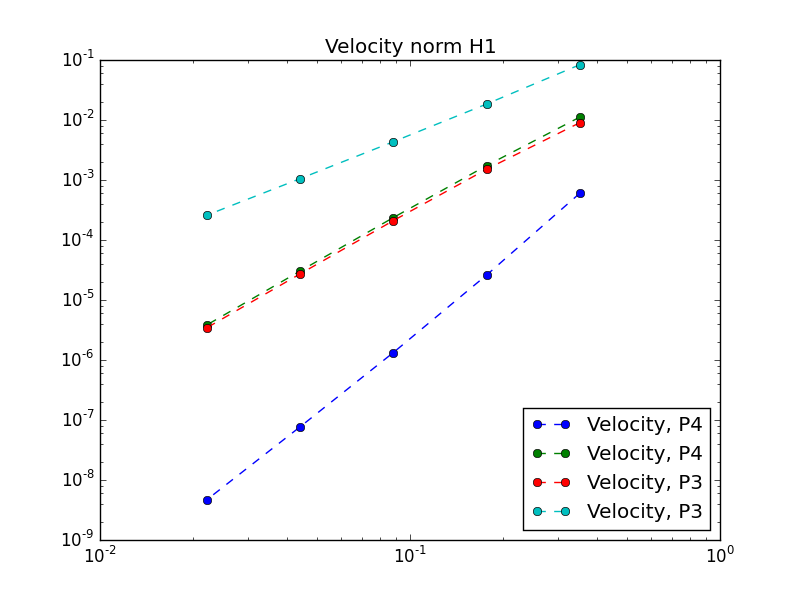
\includegraphics[scale=0.36]{velocity.png}
		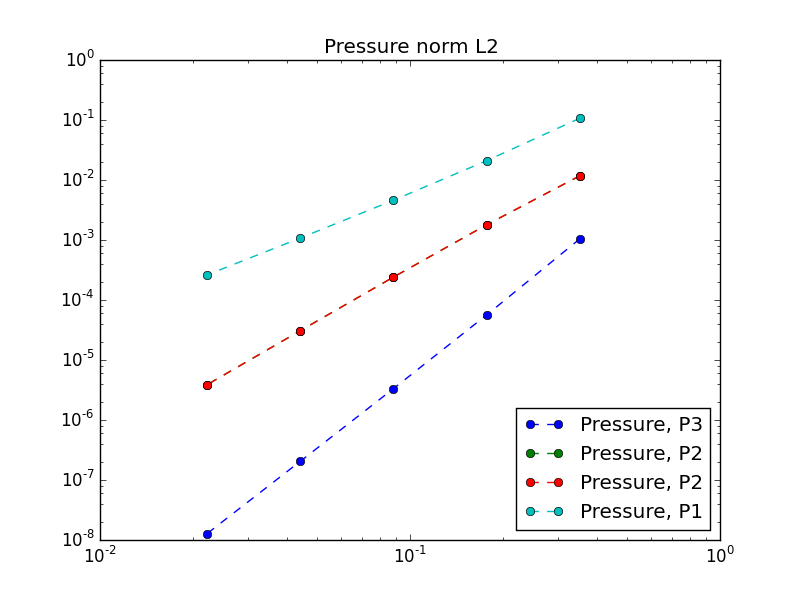
\includegraphics[scale=0.36]{pressure.png}
\end{figure}

\begin{figure}[h!]
	\centering
	\caption*{loglogplot}
	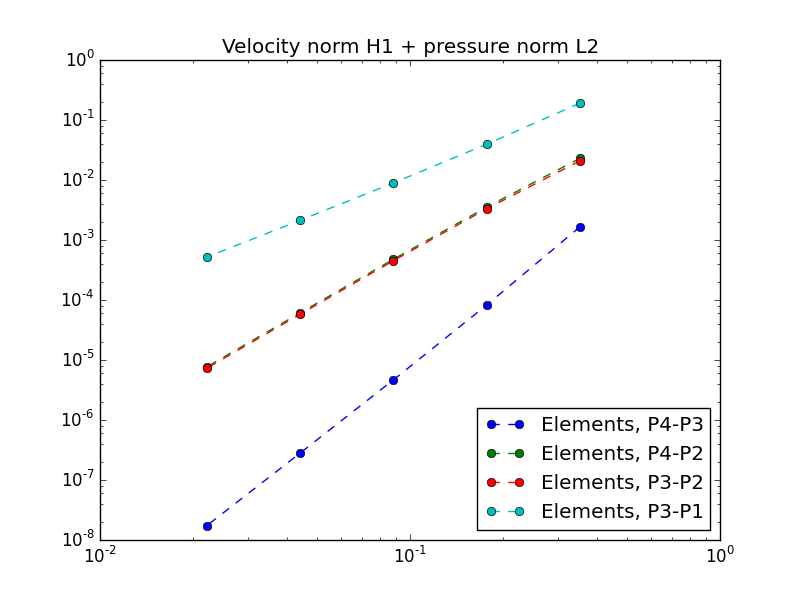
\includegraphics[scale=0.5]{comb.png}
\end{figure}

\newpage
\subsection{Exercise 7.7}
In this exercise we where to calculate the order of convergence for the shear stress in the same domain presented en exercise 7.6.
Let \textit{P} denote the stress tensor. The wall stress on a surface in the domain is given by $\textit{P} \cdot \textbf{n}$, where \textbf{n} is the normal vector
pointing perpendicular to the surface out of the domain. Hence we have the following relations

\begin{align*}
 &\textbf{\textit{P}}_n = \textit{P} \cdot \textbf{n} \hspace{12mm} \text{Shear stress} \\
	&P_{nn} = \textbf{n} \cdot \textbf{\textit{P}}_n \hspace{8mm} \text{Normal stress component} \\
	&P_{nt} = |\textbf{\textit{P}}_n \times \textbf{n}| \hspace{5mm} \text{Tangential stress component}
	\end{align*}

In this exercise we are interested in the wall shear stress, hence we will for this time focus on the tagential stress.
It can be shown that the tagential stress on a wall, perpendicular to the y-axis can be written as
$\tau = \mu \frac{\partial u}{\partial y}$. We will use the same parameters in the previous exercise in the numerical
calculations. My result yields.

\begin{table}[ht]
\caption {L2 norm wall shear stress}
\centering
\begin{tabular}{c|cccc}
\hline
\rowcolor{LightCyan}
N  &  8  &  16  &  32 &  64\\
\hline
4-3 & 3.62512e-05 & 2.35592e-06 & 1.50416e-07 & 9.47586e-09 \\ \hline
4-2 & 0.00218017  & 0.000283408 & 3.55504e-05 & 4.42797e-06 \\ \hline
3-2 & 0.00118138  & 0.00014241  & 1.6705e-05  & 1.98931e-06 \\ \hline
3-1 & 0.0217495   & 0.00446278  & 0.00100643  & 0.000242272 \\
\hline
\end{tabular}
\end{table}

\begin{table}[ht]
\caption {Convergence rate wall shear stress}
\centering
\begin{tabular}{c|ccc}
\hline
\rowcolor{LightCyan}
N  & Conv 8 to 16  &  Conv 16 to 32 &  Conv 32 to 64 \\
\hline
4-3 & 3.94367 & 3.96926 & 3.98856   \\ \hline
4-2 & 2.94349 & 2.99494 & 3.00515  \\ \hline
3-2 & 3.05234 & 3.0917  & 3.06995  \\ \hline
3-1 & 2.28497 & 2.1487  & 2.05454  \\
\hline
\end{tabular}
\end{table}

\begin{figure}[h!]
	\centering
	\caption*{loglogplot}
	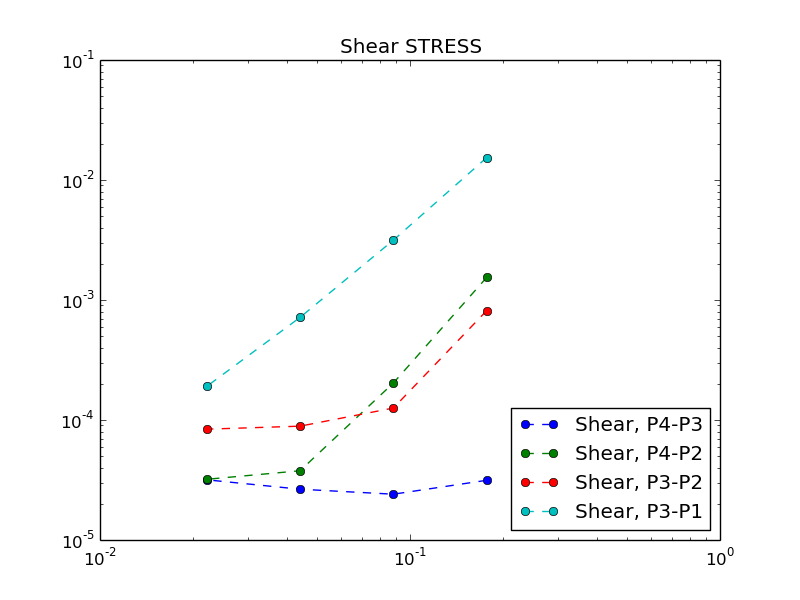
\includegraphics[scale=0.4]{shear.png}
\end{figure}

As we can see, the inital look on the convergence rate something feels wrong. Even though we used the $L_2$ norm
to compute error, we observe that the convergence rate follows the trend of a $H_1$ norm. It is important to take a closer of what
we compute the errornorm of. As we can see the wall shear stress is calculated using the derivative of the velocity \textbf{u}, as does the $H^1$ norm. As a consequence the convergence rate is limited to the same order as we saw in the previous exercise.


\section*{Exersize 2, Linear Elasticity}
In this exercise we are to take a closer look on linear elasticity, and familiarize ourselfs with
the numerical artifact locking. We are presented with the following problem

\begin{align*}
-\mu \Delta \textbf{u} - \lambda \nabla \nabla \cdot \textbf{u} = \textbf{f} \hspace{2mm} \text{in} \hspace{2mm} \Omega \\
\textbf{u} = u_e \hspace{2mm} \text{on} \hspace{2mm} \partial \Omega \\
u_e = \big(\frac{\partial \phi}{\partial y}, -\frac{\partial \phi}{\partial x} \big) \hspace{3mm}
\phi = sin(\pi x y)
\end{align*}

First and foremost since we are makeing a "manufactured solution", we need to determine the sourceterm \textbf{f}. The equation
to solve for \textbf{f} is $\textbf{f} =\mu  \Delta \textbf{u}_e$, due to by construction $\nabla \cdot \textbf{u}_e = 0$
 Hand calculations and verification with sympy gives us the following result.

\begin{align*}
\textbf{f} = \mu \big(\pi^3 x^3 cos(\pi x y) -\pi^2y (2sin(\pi x y) + \pi x y cos(\pi x y)   ) \big) \textbf{i} \hspace{1mm} + \\
\mu \big( \pi^3y^3 cos(\pi x y) + \pi^2 x (2 sin(\pi x y) + \pi x y cos(\pi x y)   ) \textbf{j} \big)
\end{align*}
Now how do we assess the problem?
Why not try stright forward Galerkin method on the problem, since we have had many good results with this approach.
Firstly lets try not alter the second term of the problem $\lambda \nabla \nabla \cdot \textbf{u}$ by integration by parts.
This gives us the following variational form.

\begin{align*}
\mu \int \Delta u v \hspace{1mm} dx + \lambda \int \nabla \nabla \cdot u v \hspace{1mm} dx = \int f v dx\\
\mu \langle \nabla u_h \,, \nabla v_h \rangle + \lambda \langle \nabla \nabla \cdot u_h \,, v_h \rangle
= \langle f \,, v \rangle
\end{align*}

Now for our numerical calulations, the problem will be solved on a UnitSquareMesh(N,N) for $N = [8, 16, 32, 64]$, for
choices of $\lambda = [1, 10, 100, 1000, 10000]$. We choice second order polynomials for the velocity. We get the following
results.

\begin{table}[ht]
\caption {L2 norm velocity}
\centering
\begin{tabular}{c|cccc}
\hline
\rowcolor{LightCyan}
$\lambda$ / N  & 8 & 16 & 32 & 64\\
\hline
1     & 0.0150549 & 0.00395643 & 0.0010022 & 0.000251384 \\ \hline
\rowcolor{LightCyan} \hline
10    & 0.725734  & 0.691357   & 0.0265754 & 0.00636318  \\ \hline
100   & 3.74994   & 0.60609    & 0.650818  & 2.41641     \\ \hline
\rowcolor{LightCyan} \hline
1000  & 2.08857   & 0.823341   & 1.16562   & 0.514192    \\ \hline
10000 & 1.42648   & 1.68109    & 3.95778   & 1.14378   \\
\hline
\end{tabular}
\end{table}

\begin{table}[ht]
\caption {Convergence rate velocity}
\centering
\begin{tabular}{c|cccccc}
\hline
\rowcolor{LightCyan}
$\lambda$ / N  & Conv 8 to 16  &  Conv 16 to 32 &  Conv 32 to 64\\
\hline
1     & 1.92796   & 1.98104   & 1.9952   &  \\ \hline
10    & 0.0700103 & 4.70127   & 2.06227  &  \\ \hline
100   & 2.62926   & -0.10272  & -1.89254 &  \\ \hline
1000  & 1.34296   & -0.501529 & 1.18071  &  \\ \hline
10000 & -0.236928 & -1.2353   & 1.79089  & \\ \hline
\end{tabular}
\end{table}

As we can see, the first run with $\lambda = 1$ gives us reasonable results. The $L_2$ norm decreases nicely for finer mesh
resolution, and the convergence rate approaches 2 which is reasonable. For $\lambda = 10$ we observe the same trend the $L_2$ norm, but allredy we observe some strange fluctations in the converegence rate.
As $\lambda$ gets bigger, we definatly see that the error gets worse. Same goes for the convergence rate. This observation of failure to converge towards the solution, as well as poor $L_2$ norm, is explained by a numerical artifact called \textit{locking}. As $\lambda$ gets bigger the material reaches an
incompressible state, where the displacements in the material gets small.
These elements we are using doesn't approximate the divergence fairly well, hence as the
$\lambda \nabla \nabla \cdot \textbf{u}$ term gets bigger, the error from the divergence pollutes our numerical results. Take for
instance $\lambda = 100$ and $N = 32$.
\begin{figure}[h!]
	\centering
	\caption*{Locking VS Exact solution $\lambda = 100$, $N = 32$}
	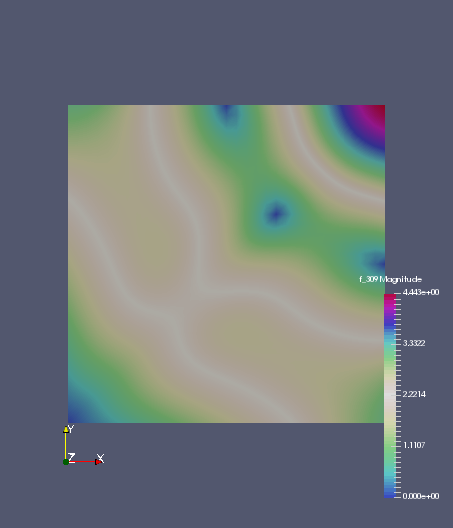
\includegraphics[scale=0.4]{lock.png}
	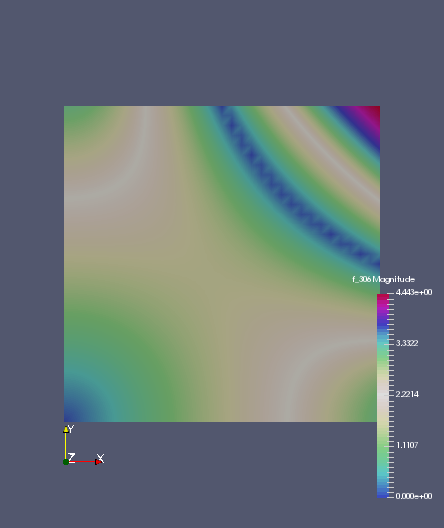
\includegraphics[scale=0.4]{exnolock.png}
\end{figure}


Now, let us try to improve our results by using integration by parts on the divergenve term.
Integration by parts gives us the following variational form and numerical results.

\begin{align*}
\mu \int \Delta u v \hspace{1mm} dx - \lambda \int \nabla \nabla \cdot u v \hspace{1mm} dx = \int f v dx\\
\mu \langle \nabla u_h \,, \nabla v_h \rangle + \lambda \langle \nabla \cdot u_h \,, \nabla \cdot v_h \rangle
= \langle f \,, v \rangle
\end{align*}
Now for our numerical calulations, the problem will be solved using the same
UnitSquareMesh(N,N)  for the same physical edentities.


\begin{table}[ht]
\caption {L2 norm velocity}
\centering
\begin{tabular}{c|cccc}
\hline
\rowcolor{LightCyan}
$\lambda$ / N  & 8 & 16 & 32 & 64\\
\hline
 1     & 0.000662282 & 4.40431e-05 & 2.81081e-06 & 1.76953e-07 \\ \hline
 \rowcolor{LightCyan}
10    & 0.00290596  & 0.000209755 & 1.38052e-05 & 8.78212e-07 \\ \hline
100   & 0.0142522   & 0.00147779  & 0.000115406 & 7.83639e-06 \\ \hline
\rowcolor{LightCyan} \hline
1000  & 0.0269102   & 0.00513695  & 0.000689253 & 6.3586e-05  \\ \hline
10000 & 0.029816    & 0.00716993  & 0.00157688  & 0.000272168 \\
\hline
\end{tabular}
\end{table}

\begin{table}[ht]
\caption {Convergence rate velocity}
\centering
\begin{tabular}{c|cccccc}
\hline
\rowcolor{LightCyan}
$\lambda$ / N  & Conv 8 to 16  &  Conv 16 to 32 &  Conv 32 to 64\\
\hline
1     & 3.91046 & 3.96985 & 3.98955 &  \\ \hline
\rowcolor{LightCyan} \hline
10    & 3.79224 & 3.92542 & 3.9745  &  \\ \hline
100   & 3.26967 & 3.67864 & 3.88039 &  \\ \hline
\rowcolor{LightCyan} \hline
1000  & 2.38917 & 2.89781 & 3.43825 &  \\ \hline
10000 & 2.05606 & 2.18488 & 2.53451 & \\
\hline
\end{tabular}
\end{table}
The numerical results have clearly improved. The $L_2$ norm have decreased, and our convergencerate have increased due
to the fact that we are now evaluating first derivatives of the velocity \textbf{u}, and not the second derivative
as we did in the naive approach. Still we observe traces of locking for higher values of $\lambda$ as we see that the $L_2$
norm and the convergence rate decreases.


\textbf{Workaround}
So is there a way to avoid \textit{locking}? Clairy we have to do something about the $\lambda \nabla \nabla \cdot \textbf{u}$ term as this ruins our numerical efforts.
One approach to limit the effects from this numerical artifact is to rewrite
the problem by introducing a mixedfunctionspace, in such a way that.

\begin{align*}
p =  \lambda \nabla \cdot \textbf{u}
\end{align*}
This simple but powerfull rewriting of the problem transforms our system written as
\begin{align*}
-\mu \Delta \textbf{u} - \nabla p = \textbf{f} \\
\nabla \cdot \textbf{u} = \frac{p}{\lambda}
\end{align*}
The familiar set of equations resembles a similar problem of the Stokes problem. Which
can be solved using Stokes stable elements,$P2-P1$ elements for the velocity and
pressure. This system of equations effects our variatonal form as follows.

\begin{align*}
\mu \langle \nabla u_h \,, \nabla v_h \rangle + \langle p \,, \nabla \cdot v \rangle = \langle f \,, v \rangle \\
\lambda \langle \nabla \cdot u \,, q \rangle - \langle p \,, q \rangle = 0
\end{align*}

We will again solve this problem, the problem will be solved on a UnitSquareMesh(N,N) for $N = [8, 16, 32, 64]$, for
choices of $\lambda = [1, 10, 100, 1000, 10000]$.

\begin{table}[ht]
\caption {L2 norm velocity}
\centering
\begin{tabular}{c|ccccc}
\hline
\rowcolor{LightCyan}
$\lambda$ / N  & 8 & 16 & 32 & 64\\
\hline
1     & 0.000350744 & 2.30646e-05 & 1.46642e-06 & 9.22282e-08 \\ \hline
\rowcolor{LightCyan} \hline
10    & 0.000352729 & 2.29796e-05 & 1.45951e-06 & 9.19713e-08 \\ \hline
100   & 0.000389985 & 2.54407e-05 & 1.62708e-06 & 1.03417e-07 \\ \hline
\rowcolor{LightCyan}
1000  & 0.000398393 & 2.60367e-05 & 1.66973e-06 & 1.0645e-07  \\ \hline
10000 & 0.000399331 & 2.61038e-05 & 1.67457e-06 & 1.06797e-07 \\
\hline
\end{tabular}
\end{table}

\begin{table}[ht]
\caption {L2 norm convergence rate}
\centering
\begin{tabular}{c|cccc}
\hline
\rowcolor{LightCyan}
$\lambda$ / N  & Conv 8 to 16  &  Conv 16 to 32 &  Conv 32 to 64 \\
\hline
1     & 3.92667 & 3.97531 & 3.99095 &  \\ \hline
\rowcolor{LightCyan} \hline
10    & 3.94014 & 3.9768  & 3.98816 &  \\ \hline
100   & 3.93821 & 3.96678 & 3.97574 &  \\ \hline
\rowcolor{LightCyan} \hline
1000  & 3.93558 & 3.96286 & 3.97136 &  \\ \hline
10000 & 3.93525 & 3.9624  & 3.97085 &  \\
\hline
\end{tabular}
\end{table}
Jugding from the results, we seemed to have found a workaround . Low $L^2$ norms combined with satisfactory
convergence, gives a good verification that the solution method is a good approximation of the system.

\end{document}
